\section{Reducing the memory usage}
\label{sec:reducing_memory}

After optimizing the detection performance, the memory usage was still to high to provide an useful alternative/boosting algorithm to the ExemplarSVM algorithm. To minimize the memory overhead, several approaches were developed and evaluated. These approaches include different storage mechanisms as kd-tree, spares matrices or plain index-value pairs and also different search and reconstruction strategies.

\subsection{Sparse matrices}

One approach is to use sparse matrices as provided by the \MATLAB framework\footnote{\url{https://de.mathworks.com/help/matlab/ref/sparse.html}}. The usage seemed to be very promising, as partial inspections of the integral images showed that approx. 70\% of the cells in a $512\times500\times375$ matrix are filled with zeros.

It showed that the \MATLAB implementation of sparse matrices is restricted to two-dimensional matrices, it is therefore required to reduce the amount of dimensions of the matrix at store time and restore the original format at runtime, or transform the required coordinates into a single index. As the internal representation of an image consists of four matrix dimensions (scale range, codebook dimensions, width, height), a matrix will be transformed into a matrix of the form $CB \times N$ whereas $CB$ is the amount of codebook dimensions and $N$ the product of the image width, height and number of scale ranges included in this matrix (usually one per saved \MATLAB file). The corresponding source code could be seen in \lstref{storage_method_sparse} in line 171. The variable \verb|si| represents the current scale ranges which will be saved. A complete reconstruction to the original, internal representation could be done with \lstref{reconstruct_sparse_matlab}. This is done by converting the sparse matrix into a full matrix containing the zero values. The new matrix is then reordered into its original four dimensional representation.

\begin{lstlisting}[firstnumber=165,caption={Sparse storage method (get\_codebook\_integrals.m)},label=lst:storage_method_sparse]
I2 = I(si, :, :, :);
Is = size(I2);
integrals(si, fi).I_size = Is;
if params.naiive_integral_backend
    integrals(si, fi).I = I2;
elseif params.integral_backend_matlab_sparse
    integrals(si, fi).I = sparse(squeeze(I2(:, :, :)));
\end{lstlisting}

\begin{lstlisting}[firstnumber=29,caption={Sparse reconstruction by \MATLAB (getCodebookIntegrals.m)},label=lst:reconstruct_sparse_matlab]
I = full(integralImg.I);
I = reshape(I, integralImg.I_size);
\end{lstlisting}

The matrices are stored in a \MATLAB file with the 7.3\footnote{A comparison table could be found at \url{https://de.mathworks.com/help/matlab/ref/save.html\#input_argument_version} (visited on 10/12/2015)} file format (required to store variables with more than two gigabytes of data).
For example the representation of the pascal image \textit{2007\_008932.jpg} containing feature patches with a maximum size of $86\times86$ pixels and 512 codebook dimensions results in a total \ac{RAM} size of 768,001,438 bytes (or 732.4 megabytes). The saved \MATLAB file occupies 6,325,415 bytes (6 megabytes) of disk space.
Stored as a sparse matrix the data is reduced to 423,905,670 bytes (404.3 megabytes or 55\%) in \ac{RAM}. After saving to a file, a size of 22,612,163 bytes (21.6 megabytes) still remains. Compared to the na\"{\i}ve (saving the matrices as is) storage method it requires 16,286,748 bytes more (15.5 megabytes or 357\%) disk space. The reason for this storage overhead could probably be found in the mandatory compression which comes with file formats greater or equal to version 7.0. For the na\"{\i}ve format, the compression can benefit from the low entropy coming from the high amount of zeros which exists in a sequential ordering. In contrast to the sparse variant, which have to compress multiple lists of coordinates and their corresponding values. Besides the fact that disk storage is a cheap resource nowadays, it also affects the loading time as more data has to be loaded. Although the decompression time could be reduced as a much lesser compression ratio was achieved. Together with the additional matrix reconstruction described above, a small speedup was still achieved whilst the memory usage was reduced by 50\%.

\subsection{Reconstructing from changing points}

As the internal representation is based on integral images, additional information can be interfered from on specific points in the matrix. Integral images are constructed by summing up values from the top left to the bottom right. This means that as long as no further points exists in the source image, the most current value is carried on until the next point is found. The example in \figref{integral_image_interference} shows and describes the behavior. As one can see, the minimum required information to construct a full integral image are the values at the points $(2,9)$, $(3,4)$, $(5,6)$ and $(5,8)$. In contrast to the sparse matrix approach, only 4 points have to be stored compared to 58 points.

Obviously the computation effort during the query search increases as the integral image would had to be computed at runtime. By sorting the points according to the sum of their coordinate values, the computation overhead could be reduced as the amount of cells which have to be summed up decreases with every point processed.
%TODO timings + memory

%\begin{lstlisting}[firstnumber=229,caption={Coordinate based storage method (get\_codebook\_integrals.m)},label=lst:storage_method_coordinate]
%[cb, x, y] = ind2sub(Is(2:end), find(remaining));
%coords = [x, y, cb];
%
%sum_values = coords(:, 1) + coords(:, 2);
%[~, idx] = sort(sum_values);
%coords = coords(idx, :);
%scores = scores(idx, :);
%
%integrals(si, fi).coords = coords;
%integrals(si, fi).scores = scores;
%\end{lstlisting}

To find a trade-off between low memory usage and computation effort, another approach came up. In this approach every changing value in the integral image is stored instead of the original values. In the current example the points $(2,9)$, $(3,4)$, $(3,9)$, $(5,6)$, $(5,8)$ and $(5,9)$ would be selected. By storing the additional points, which were created at the intersection points of the original ones, we are able to reconstruct the full matrix by taking the list of points, sorting them by the sum of their coordinates and writing one point at a time from its position to the bottom right. In the current example the list would be sorted as \mathlist{(3,4), (5,6), (2,9), (3,9), (5,8), (5,9)}. In the first step the point $(3,4)$ would be selected and its value ($2$) would be written to the bottom right as shown in \figref{integral_image_interference2:point1}. The second step selects point $(5,6)$ and write its value $5$ in the same way as before.
This technique will be applied to all points in the list until the integral image is fully reconstructed.
The speed up comparing to the previous approach is based on the fact that no memory read from any cell has to be made and no arithmetic instruction has to be executed. The limiting factor in this case is ability to write values fast at specific positions in \ac{RAM}.
%TODO timings + memory

\begin{figure}
\begin{subfigure}{.5\textwidth}
    % !TeX root = ../../main.tex
\resizebox{\textwidth}{\textwidth}{
    \tikzsetnextfilename{source_image}
    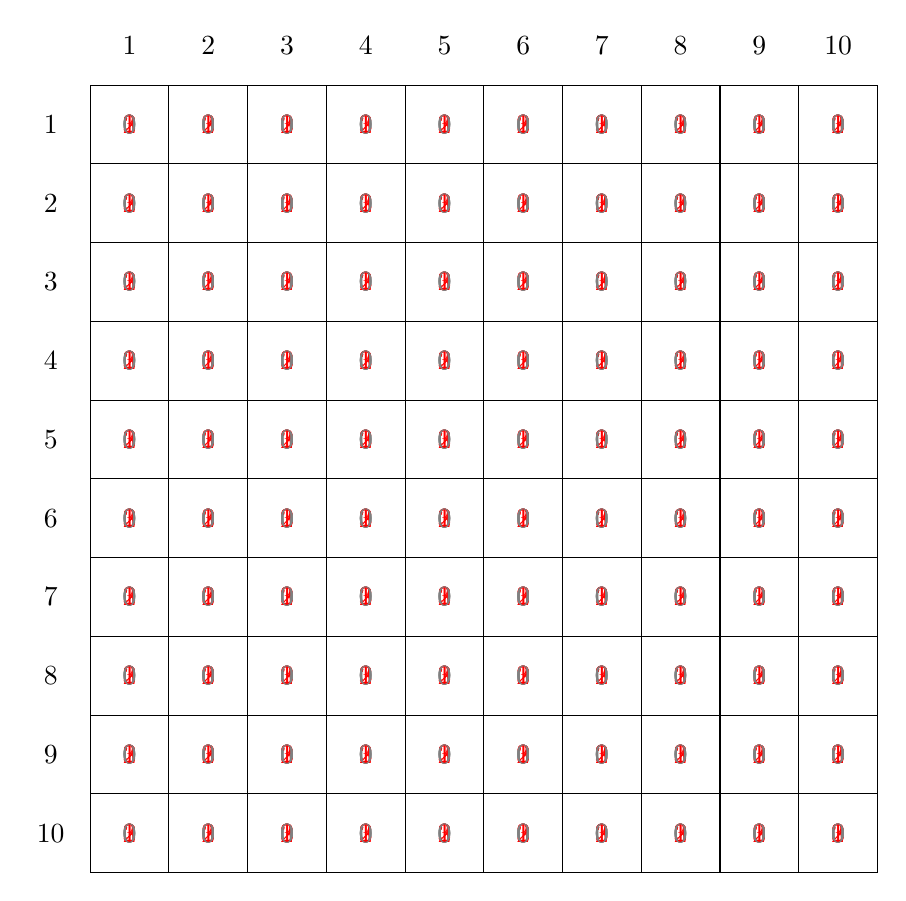
\begin{tikzpicture}
    \foreach \x in {1,...,10} {
        \draw (\x + 0.5, 11.5) node {\x};
    }
    \foreach \y in {10,...,1} {
        \draw (0.5, 11.5 - \y) node {\y};
    }
    \foreach \x in {1,...,10} {
        \foreach \y in {1,...,10} {
            \draw (\x, \y) rectangle (\x +1, \y +1);
            \ifnumequal{\x}{5}{
                \ifnumequal{\y}{5}{
                    \draw[color=red] (\x +0.5, \y +0.5) node {3};
                }{
                    \ifnumequal{\y}{3}{
                        \draw[color=red] (\x +0.5, \y +0.5) node {2};
                    }{
                        \draw[color=gray] (\x +0.5, \y +0.5) node {0};
                    }
                }
            }{
                \ifnumequal{\x}{2}{
                    \ifnumequal{\y}{2}{
                        \draw[color=red] (\x +0.5, \y +0.5) node {1};
                    }{
                        \draw[color=gray] (\x +0.5, \y +0.5) node {0};
                    }
                }{
                    \ifnumequal{\x}{3}{
                        \ifnumequal{\y}{7}{
                            \draw[color=red] (\x +0.5, \y +0.5) node {2};
                        }{                    
                            \draw[color=gray] (\x +0.5, \y +0.5) node {0};
                        }
                    }{
                        \draw[color=gray] (\x +0.5, \y +0.5) node {0};
                    }
                }
            }
        }
    }
    \end{tikzpicture}
}
    \caption{Source image}
    \label{fig:integral_image_interference:source_image}
\end{subfigure}%
\begin{subfigure}{.5\textwidth}
    % !TeX root = ../../main.tex
 \resizebox{\textwidth}{\textwidth}{
     \tikzsetnextfilename{integral_image}
    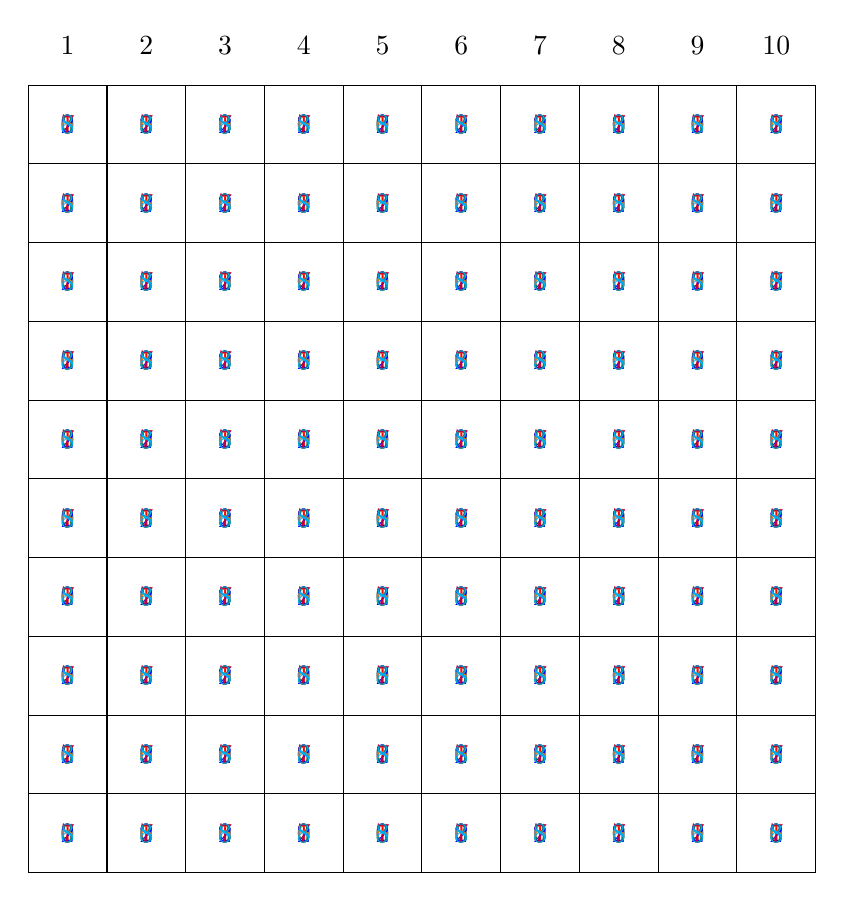
\begin{tikzpicture}
    \foreach \x in {1,...,10} {
        \draw (\x + 0.5, 11.5) node {\x};
    }
    \foreach \x in {1,...,10} {
        \foreach \y in {1,...,10} {
            \draw (\x, \y) rectangle (\x +1, \y +1);
            \ifnumcomp{\x}{<}{2}{
                \draw[color=gray] (\x +0.5, \y +0.5) node {0};
            }{
                \ifnumcomp{\x}{<}{3}{
                    \ifnumcomp{\y}{>}{2}{
                        \draw[color=gray] (\x +0.5, \y +0.5) node {0};
                    }{
                        \draw[color=red] (\x +0.5, \y +0.5) node {1};
                    }
                }{
                    \ifnumcomp{\y}{>}{7}{
                        \draw[color=gray] (\x +0.5, \y +0.5) node {0};
                    }{
                        \ifnumcomp{\y}{>}{2}{
                            \ifnumcomp{\x}{<}{5}{
                                \draw[color=blue] (\x +0.5, \y +0.5) node {2};
                            }{
                                \ifnumcomp{\y}{>}{5}{
                                    \draw[color=blue] (\x +0.5, \y +0.5) node {2};
                                }{
                                    \ifnumcomp{\y}{>}{3}{
                                        \draw[color=orange] (\x +0.5, \y +0.5) node {5};
                                    }{
                                        \draw[color=purple] (\x +0.5, \y +0.5) node {7};
                                    }
                                }
                            }
                        }{
                            \ifnumcomp{\x}{<}{5}{
                                \draw[color=teal] (\x +0.5, \y +0.5) node {3};
                            }{
                                \draw[color=cyan] (\x +0.5, \y +0.5) node {8};
                            }
                        }
                    }
                }
            }
        }
    }
    \end{tikzpicture}
}
    \caption{Integral image}
    \label{fig:integral_image_interference:integral_image}
\end{subfigure}%
\caption[Creation of an integral image]{The source image in \subref{fig:integral_image_interference:source_image} contains values at the positions $(2,9)$, $(3,4)$, $(5,6)$ and $(5,8)$. As shown in \subref{fig:integral_image_interference:integral_image} their values expand to the bottom right. Even if the amount of zero values decreased, the matrix contain still a high percentage of repetitions.}
\label{fig:integral_image_interference}
\end{figure}

\begin{figure}
\begin{subfigure}{.5\textwidth}
    % !TeX root = ../../main.tex
\resizebox{\textwidth}{\textwidth}{
    \tikzsetnextfilename{reconstruct_point1}
    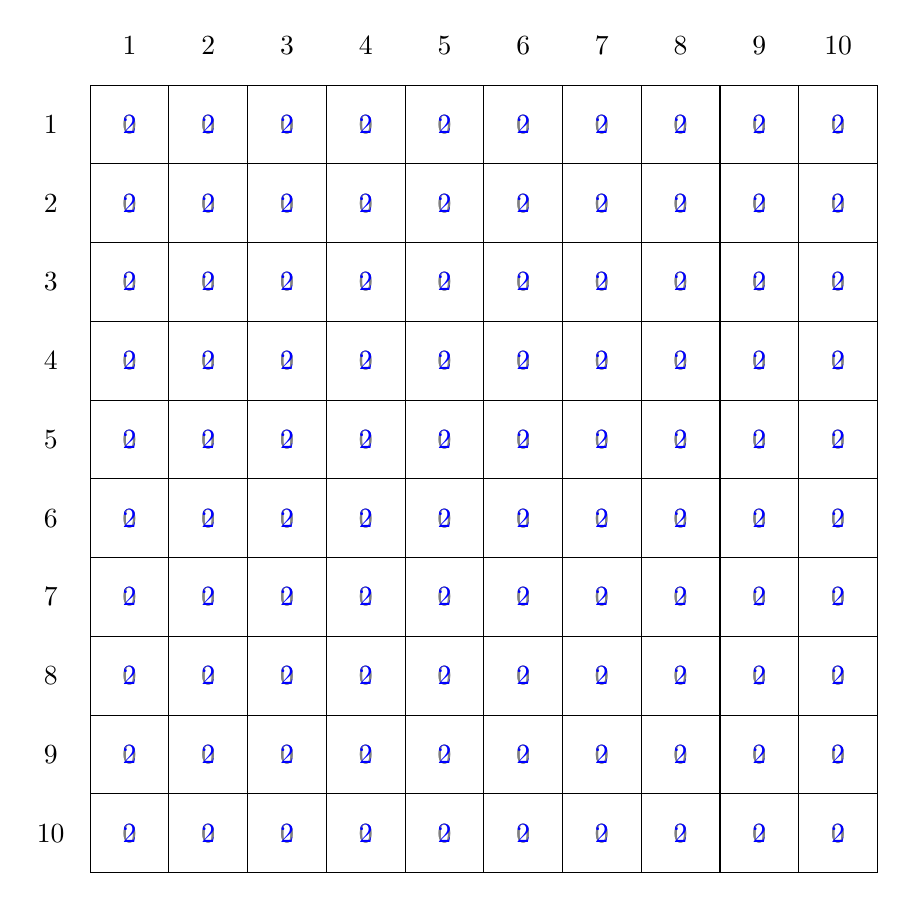
\begin{tikzpicture}
    \foreach \x in {1,...,10} {
        \draw (\x + 0.5, 11.5) node {\x};
    }
    \foreach \y in {10,...,1} {
        \draw (0.5, 11.5 - \y) node {\y};
    }
    \foreach \x in {1,...,10} {
        \foreach \y in {1,...,10} {
            \draw (\x, \y) rectangle (\x +1, \y +1);
            \ifnumcomp{\x}{<}{3}{
                \draw[color=gray] (\x +0.5, \y +0.5) node {0};
            }{
                \ifnumcomp{\y}{>}{7}{
                    \draw[color=gray] (\x +0.5, \y +0.5) node {0};
                }{
                    \draw[color=blue] (\x +0.5, \y +0.5) node {2};
                }
            }
        }
    }
    \end{tikzpicture}
}
    \caption{Reconstructing point $(3,4)$}
    \label{fig:integral_image_interference2:point1}
\end{subfigure}%
\begin{subfigure}{.5\textwidth}
    % !TeX root = ../../main.tex
\resizebox{\textwidth}{\textwidth}{
    \tikzsetnextfilename{reconstruct_point2}
    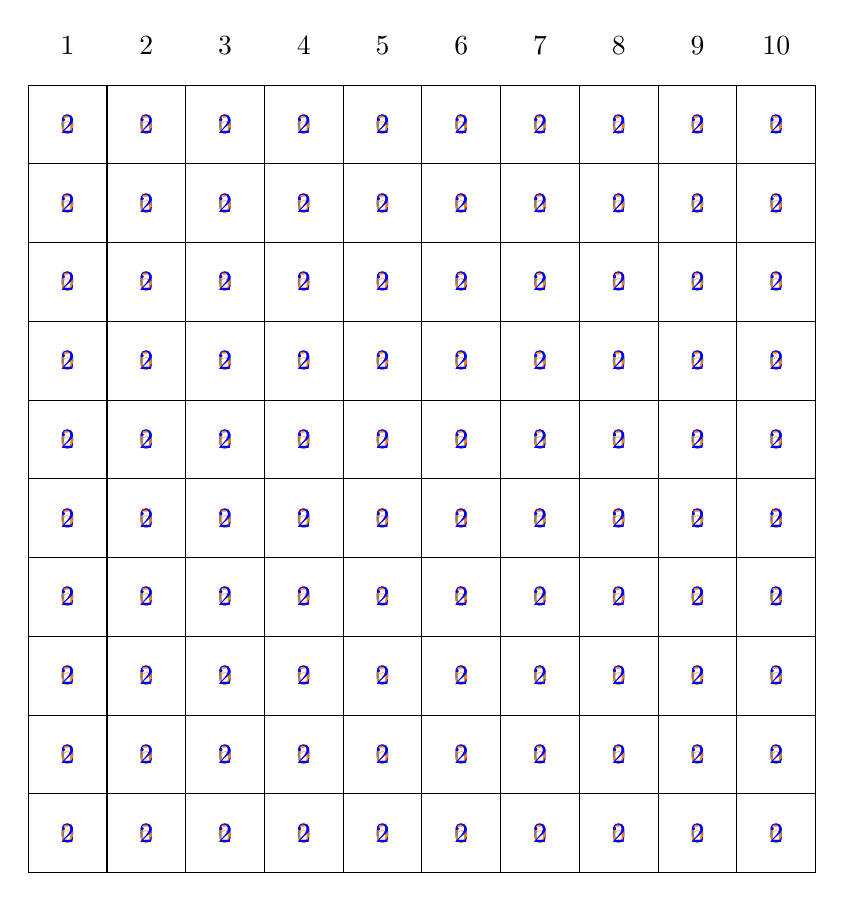
\begin{tikzpicture}
    \foreach \x in {1,...,10} {
        \draw (\x + 0.5, 11.5) node {\x};
    }
    \foreach \x in {1,...,10} {
        \foreach \y in {1,...,10} {
            \draw (\x, \y) rectangle (\x +1, \y +1);
            \ifnumcomp{\x}{<}{3}{
                \draw[color=gray] (\x +0.5, \y +0.5) node {0};
            }{
                \ifnumcomp{\y}{>}{7}{
                    \draw[color=gray] (\x +0.5, \y +0.5) node {0};
                }{
                    \ifnumcomp{\y}{<}{6}{
                        \ifnumcomp{\x}{>}{4}{
                            \draw[color=orange] (\x +0.5, \y +0.5) node {5};
                        }{
                            \draw[color=blue] (\x +0.5, \y +0.5) node {2};
                        }                                                    
                    }{
                        \draw[color=blue] (\x +0.5, \y +0.5) node {2};
                    }                      
                }
            }
        }
    }
    \end{tikzpicture}
}
    \caption{Reconstructing point $(5,6)$}
    \label{fig:integral_image_interference2:point2}
\end{subfigure}%
\caption{Reconstructing integral image from intersection points}
\label{fig:integral_image_interference2}
\end{figure}

The fourth approach tried to achieve an additional reduction of the writing cycles. This is done by storing additional points, which are selected by scanning the integral image row by row. Each time a value change is detected, the point is added to the list. In the example the complete list would be noted as \mathlist{(3,4), (3,5), (3,6), (5,6), (3,7), (5,7), (3,8), (5,8), (2,9), (3,9), (5,9), (2,10), (3,10), (5,10)}. In the reconstruction phase, the algorithm jumps at the first point for each row and writes its value to the right until he reaches the next point in the list. Now the new value is written to right until the next point is reached and so forth.
%TODO timings + memory

The fifth approach skips the reconstruction completely and tries to find any value by searching in the list of intersection values from the third approach. In the initial implementation, the scores were stored aside to their x, y and codebook dimension coordinates ($img_x$, $img_y$ and $img_{codebook}$ respectively). The actual search consisted of three steps. In the first step, all coordinates and values are selected which correspond to the lower or equal x values compared to the query x value ($query_x$). Within the subset all values belonging to $img_y \le query_y$ are selected. The resulting subset is scanned from lower to higher coordinates (sorted by $img_x$, $img_y$ and $img_{codebook}$) and will fill a codebook based on the $img_{codebook}$ and score values. %TODO laufzeit fuer alle suchen angeben (O(...))

As one may notice this represents more or less multiple linear searches, which has to be done by every requested codebook at a specific point. To speedup the search a binary searching algorithm based on kd-trees were implemented. %TODO binary search, kd-tree erklaeren
Instead of filtering by the x and y coordinates first and filling the codebook with the last changed values, the filtering for this approach was reversed. Every integral image is represented by as many kd-trees as codebook dimensions exist. If one codebook dimension is never used throughout the while image, the corresponding tree will be empty. Each of the remaining trees consist of two matrices. The first matrix contains three rows with as many columns as unique x coordinates for this codebook dimension exist. The first row contains the current x coordinate, the second the starting index for the second matrix and the third row the end index for the second matrix. The second matrix consists of two rows. One containing all y coordinates and the other all scores.

When searching a value for a specific codebook dimension at a specific point, the kd-tree which corresponds to the codebook dimension is selected. Within the first matrix the highest x value lower or equal to $query_x$ is searched and the second matrix is cut to the start and end indices extracted from the first matrix. Within this smaller matrix the highest y value lower or equal to $query_y$ is searched and the corresponding score is used as the codebook dimension value. Both searches can be done by a binary search approach in $O(\log_2 N)$. Additionally, most of the searches will be canceled early, as either the codebook dimension is empty, the $query_x$ is outside of the x values or $query_y$ is outside of the y values. %TODO nachweis????
%TODO timings + memory

%\begin{lstlisting}[firstnumber=179,caption={KD-Tree storage method (get\_codebook\_integrals.m)},label=lst:storage_method_kdtree]
%remaining = I2 ~= 0;
%
%I2 = I2(remaining);
%scores = I2(:);
%if params.use_kdtree
%    [cb, x, y] = ind2sub(Is(2:end), find(remaining));
%    % sort order: y x cb
%    coords = [cb, x, y];
%    cb = unique(cb);
%    cblen = length(cb);
%    if cblen > 0
%        tmptree = alloc_struct_array(cblen, 'x', 'y');
%        parfor ci=1:cblen
%            dim = cb(ci);
%            if ci == 1 || ci == cblen || mod(ci, 100) == 0
%                debg('[%4d/%04d] Dimension %d', ci, cblen, dim);
%            end
%            cs = coords(:, 1) == cb(ci);
%            x = coords(cs, 2);
%            y = coords(cs, 3);
%            s = scores(cs);
%            ux = unique(x);
%            data2 = zeros([length(ux) 3], 'uint32');
%            data2(:, 1) = ux;
%            data3 = zeros([length(y) 2]);
%            from = 1;
%            to = 0;
%            for xi=1:length(ux)
%                xs = x == ux(xi);
%                sxs = sum(xs);
%                if sxs
%                    to = to + sum(xs);
%                    data3(from:to, 1) = y(xs);
%                    data3(from:to, 2) = s(xs);
%                    data2(xi, [2 3]) = [from, to];
%                    from = to+1;
%                end
%            end
%            tmptree(ci).x = data2;
%            tmptree(ci).y = data3;
%        end
%        tree = alloc_struct_array(Is(2), 'x', 'y');
%        tree(cb) = tmptree;
%    else
%        tree = alloc_struct_array(Is(2), 'x', 'y');
%    end
%
%    %tree = create_kd_tree(cb, tree);
%    integrals(si, fi).tree = tree;
%\end{lstlisting}

% kd - tree
% sparse matrix
% overwrite
% sum